% Very simple template for lab reports. Most common packages are already included.
\documentclass[a4paper, 11pt]{article}
\usepackage[utf8]{inputenc} % Change according your file encoding
\usepackage{graphicx}
\usepackage{url}
\usepackage{caption}
\usepackage{subcaption}

\title{\textbf{Distributed Artificial Intelligence and Intelligent Agents Homework 1}}
\author{KTH Royal Institute of Technology \\ 
		School of Information and Communication Technology \\
		Student:Fanti Machmount Al Samisti (fmas@kth.se) \\
		Student:Pradeep Perris (pradeep@kth.se)}

\begin{document}
	
\maketitle

\section{Introduction}

\noindent The goal of this project is to implement a distributed key-value store with many freedoms given at hand like the structure, replication algorithm and factor and much more. We chose a full graph network e.g. if \textbf{n = 4} then $K_4$(in graph theory terms). 

{\centering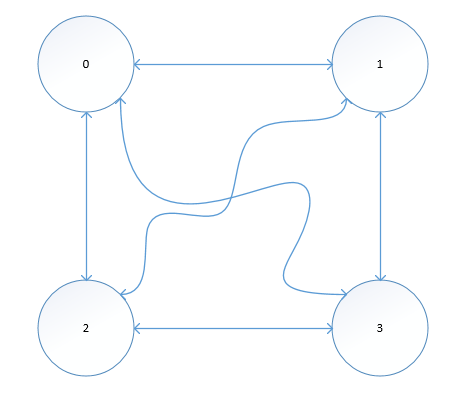
\includegraphics[scale = 0.9]{./figures/network-overview.png}\par}

\section{Enter the matrix}

\noindent The execution with \textbf{3 Nodes}, Node with 0 id is the always the initial leader:
\begin{verbatim}
INFO  {Node} [0]: Got JOIN message from ID: [1]
INFO  {Node} [0]: Got JOIN message from ID: [2]
INFO  {Node} [1]: Got VIEW message from ID: [0](0 1)
INFO  {Node} [1]: Got VIEW message from ID: [0](0 1 2)
INFO  {Node} [2]: Got VIEW message from ID: [0](0 1 2)
\end{verbatim}

\section{Configuration}

\noindent Since our network is a virtual one, we don't have to define multiple port numbers and IP addresses. Below is a concrete example of how it might look:

\begin{verbatim}
network {
    node {
        host = "127.0.0.1"
        port = 34567
    }
    grid {
        num = 3 # Size of the network, has to be at least 3
    }
}
\end{verbatim}


\section{References}
\begin{itemize}
	\item http://www.slideshare.net/WayneJonesJnr/chapter-16-distributed-system-structures-1314596
	\item 
	http://blog.fourthbit.com/2015/04/12/building-a-distributed-fault-tolerant-key-value-store
\end{itemize}

\end{document}
